\documentclass[10pt,fleqn]{article}
\mathindent 0.0in
\usepackage[utf8]{inputenc}
\usepackage{times}
\usepackage{graphicx}
\usepackage{color}
\definecolor{silver}{rgb}{0.75,0.75,0.75}
\definecolor{gray}{rgb}{0.5,0.5,0.5}
\definecolor{aqua}{rgb}{0.5,1,1}
\definecolor{navy}{rgb}{0.0,0.0,0.5}
\definecolor{orange}{rgb}{1.0,0.5,0.0}
\definecolor{teal}{rgb}{0.25,0.5,0.5}
\definecolor{olive}{rgb}{0.5,0.5,0.0}
\definecolor{purple}{rgb}{0.5,0.0,0.5}
\definecolor{brown}{rgb}{0.5,0.25,0.0}
\definecolor{fuchsia}{rgb}{1.0,0.5,1.0}
\definecolor{buff}{rgb}{1.0,0.94,0.80}
\definecolor{lime}{rgb}{0.5,1.0,0.0}
\setlength{\headsep}{-0.6in}
\setlength{\textheight}{1in}
\setlength{\footskip}{1.0 in}
\setlength{\oddsidemargin}{-0.2in}
\setlength{\evensidemargin}{-0.2in}
\setlength{\textwidth}{1.3in}
\usepackage{longtable}
\newcommand{\abs}[1]{\left|#1\right|}
\newcommand{\F}[1]{\mbox{$#1$}}
\newcommand{\K}[1]{\mbox{\sf#1\ \ \mit}}
\newcommand{\KS}[1]{\mbox{\sf\ \ #1\ \ \mit}}
\newcommand{\SC}[1]{\mbox{`#1'}\  }
\newcommand{\V}[1]{\mbox{$ #1 $}}
\newcommand{\I}{\mbox{\hspace{0.20in}}}
\newcommand{\temperature}{\mathrm{T}}
\newcommand{\pressure}{\mathrm{P}}
\newcommand{\volume}{\mathrm{v}}
\newcommand{\density}{\mathrm{\rho}}
\newcommand{\intenergy}{\mathrm{u}}
\newcommand{\enthalpy}{\mathrm{h}}
\newcommand{\entropy}{\mathrm{s}}
\newcommand{\molarmass}{\mathrm{MW}}
\newcommand{\enthalpyfusion}{\mathrm{\Delta h_{fusion}}}
\newcommand{\enthalpyvaporization}{\mathrm{\Delta h_{vaporization}}}
\newcommand{\quality}{\mathrm{x}}
\newcommand{\viscosity}{\mathrm{\mu}}
\newcommand{\conductivity}{\mathrm{k}}
\newcommand{\prandtl}{\mathrm{P_r}}
\newcommand{\cp}{\mathrm{c_p}}
\newcommand{\cv}{\mathrm{c_v}}
\newcommand{\specheat}{\mathrm{c_p}}
\newcommand{\soundspeed}{\mathrm{c}}
\newcommand{\wetbulb}{\mathrm{wb}}
\newcommand{\humrat}{\mathrm{\omega}}
\newcommand{\acentricfactor}{\mathrm{\omega}}
\newcommand{\relhum}{\mathrm{\phi}}
\newcommand{\dewpoint}{\mathrm{DP}}
\newcommand{\volexpcoef}{\mathrm{\beta}}
\newcommand{\compressibilityfactor}{\mathrm{Z}}
\newcommand{\surfacetension}{\mathrm{\gamma}}
\newcommand{\tcrit}{\mathrm{T_{crit}}}
\newcommand{\pcrit}{\mathrm{P_{crit}}}
\newcommand{\vcrit}{\mathrm{v_{crit}}}
\newcommand{\ttriple}{\mathrm{T_{triple}}}
\newcommand{\fugacity}{\mathrm{fugacity}}
\newcommand{\tsat}{\mathrm{T_{sat}}}
\newcommand{\psat}{\mathrm{P_{sat}}}
\newcommand{\eklj}{\mathrm{ek_{LJ}}}
\newcommand{\sigmalj}{\mathrm{\sigma_{LJ}}}
\begin{document}
\begin{center}
\bf \mbox{TALLER1}
\vspace{0.2 in}
\end{center}
\subsection*{Equations}
\begin{equation}
\label{EES Eqn:1}
M_{CO} = 28.013   \   \left[ \rm kg/kmol \right] 
\end{equation}
{\color{blue} \rm}
\begin{equation}
\label{EES Eqn:2}
M_{CO2} =  \left( 44.01 \right)    \   \left[ \rm kg/kmol \right] 
\end{equation}
{\color{blue} \rm}
\begin{equation}
\label{EES Eqn:3}
M_{H2} =  \left( 2.016 \right)    \   \left[ \rm kg/kmol \right] 
\end{equation}
{\color{blue} \rm}
\begin{equation}
\label{EES Eqn:4}
M_{CH4} =  \left( 16.043 \right)    \   \left[ \rm kg/kmol \right] 
\end{equation}
{\color{blue} \rm}
\begin{equation}
\label{EES Eqn:5}
M_{NH3} =  \left( 17.03 \right)    \   \left[ \rm kg/kmol \right] 
\end{equation}
{\color{blue} \rm}
\begin{equation}
\label{EES Eqn:6}
M_{Air} = 39   \   \left[ \rm kg/kmol \right] 
\end{equation}
{\color{blue} \rm}
\begin{equation}
\label{EES Eqn:7}
M_{H2O} = \molarmass \left(\F{H2O }\right)  
\end{equation}
\begin{equation}
\label{EES Eqn:8}
n_{CO} = 37.84\times 10^{-2}   \   \left[ \rm kmol \right] 
\end{equation}
{\color{blue} \rm}
\begin{equation}
\label{EES Eqn:9}
n_{CO2} = 19.03\times 10^{-2}   \   \left[ \rm kmol \right] 
\end{equation}
{\color{blue} \rm}
\begin{equation}
\label{EES Eqn:10}
n_{H2} = 22.72\times 10^{-2}   \   \left[ \rm kmol \right] 
\end{equation}
{\color{blue} \rm}
\begin{equation}
\label{EES Eqn:11}
n_{CH4} = 14.95\times 10^{-2}   \   \left[ \rm kmol \right] 
\end{equation}
{\color{blue} \rm}
\begin{equation}
\label{EES Eqn:12}
n_{NH3} = 5.46\times 10^{-2}   \   \left[ \rm kmol \right] 
\end{equation}
{\color{blue} \rm}
\begin{equation}
\label{EES Eqn:13}
x = n_{CO} + n_{CO2} + n_{CH4} 
\end{equation}
\begin{equation}
\label{EES Eqn:14}
2\cdot y = 2\cdot n_{H2} +  \left( 4 \right) \cdot  \left( n_{CH4} \right)  +  \left( 3 \right) \cdot n_{NH3} 
\end{equation}
\begin{equation}
\label{EES Eqn:15}
z = 2 \cdot  3.76 \cdot  a_{s} + n_{NH3} 
\end{equation}

\vspace{0.10in}
\noindent
{\color{blue} \rm Para encontrar el aire teórico balanceamos el Oxígeno}
\begin{equation}
\label{EES Eqn:16}
n_{CO} + 2\cdot n_{CO2} + a_{s}\cdot 2 = 2\cdot x + y 
\end{equation}
\begin{equation}
\label{EES Eqn:17}
n_{product} = x + y + z 
\end{equation}
\begin{equation}
\label{EES Eqn:18}
\phi = 1.2 
\end{equation}
\begin{equation}
\label{EES Eqn:19}
x_{e} = n_{CO} + n_{CO2} + n_{CH4} 
\end{equation}
\begin{equation}
\label{EES Eqn:20}
2\cdot y_{e} =  \left( 2 \right) \cdot n_{H2} +  \left( 4 \right) \cdot n_{CH4} +  \left( 3 \right) \cdot n_{NH3} 
\end{equation}
\begin{equation}
\label{EES Eqn:21}
2\cdot z_{e} = 2\cdot  3.76 \cdot  \phi \cdot  a_{s} + 1 \cdot  n_{NH3} 
\end{equation}

\vspace{0.10in}
\noindent
{\color{blue} \rm Para encontrar el aire te�rico balanceamos el Ox�geno}
\begin{equation}
\label{EES Eqn:22}
n_{CO} + 2\cdot n_{CO2} + a_{s}\cdot \phi\cdot 2 = 2\cdot x_{e} + y_{e} + 2\cdot w 
\end{equation}
\begin{equation}
\label{EES Eqn:23}
n_{product20} = x_{e} + y_{e} + z_{e} + w 
\end{equation}
\begin{equation}
\label{EES Eqn:24}
n_{CO2p} = x_{e} 
\end{equation}
\begin{equation}
\label{EES Eqn:25}
n_{H2O} = y_{e} 
\end{equation}
\begin{equation}
\label{EES Eqn:26}
n_{N2p} = z_{e} 
\end{equation}
\begin{equation}
\label{EES Eqn:27}
n_{O2p} = w 
\end{equation}
\begin{equation}
\label{EES Eqn:28}
n_{O2r} = \phi\cdot a_{s}\cdot 1 
\end{equation}
\begin{equation}
\label{EES Eqn:29}
n_{N2r} = \phi\cdot a_{s}\cdot 3.76 
\end{equation}
\begin{equation}
\label{EES Eqn:30}
T_{1} = \mbox{ConvertTemp}{ \left( C,\ K,\ 25 \right) } 
\end{equation}
\begin{equation}
\label{EES Eqn:31}
P_{1} = 1   \   \left[ \rm atm \right] \cdot  \rm { \left|101.325\ \frac {\rm{kPa}}{\rm{atm}}\right|} 
\end{equation}
{\color{blue} \rm}
\begin{equation}
\label{EES Eqn:32}
P_{2} = P_{1} 
\end{equation}
\begin{equation}
\label{EES Eqn:33}
Q_{T} = 0 
\end{equation}
\begin{equation}
\label{EES Eqn:34}
Q_{T} = n_{CO2p}\cdot \enthalpy \left(\F{CO2},\mbox{\ T}=\V{T2}  \right)  + n_{H2O}\cdot \enthalpy \left(\F{H2O},\mbox{\ T}=\V{T2}  \right)  + n_{N2p}\cdot \enthalpy \left(\F{N2},\mbox{\ T}=\V{T2}  \right)  +  n_{O2p}\cdot \enthalpy \left(\F{O2},\mbox{\ T}=\V{T2}  \right)  -  \left( n_{CO}\cdot \enthalpy \left(\F{CO},\mbox{\ T}=T_{1} \right)  + n_{CO2}\cdot \enthalpy \left(\F{CO2},\mbox{\ T}=T_{1} \right)  + n_{H2}\cdot \enthalpy \left(\F{H2},\mbox{\ T}=T_{1} \right)  + n_{CH4}\cdot \enthalpy \left(\F{CH4},\mbox{\ T}=T_{1} \right)  + n_{NH3}\cdot \enthalpy \left(\F{NH3},\mbox{\ T}=T_{1} \right)  + n_{O2r}\cdot \enthalpy \left(\F{O2},\mbox{\ T}=T_{1} \right)  + n_{N2r}\cdot \enthalpy \left(\F{N2},\mbox{\ T}=T_{1} \right)  \right)  
\end{equation}
\begin{equation}
\label{EES Eqn:35}
T_{2} = T_{1} 
\end{equation}
\begin{equation}
\label{EES Eqn:36}
Q_{max} = n_{CO2p}\cdot \enthalpy \left(\F{CO2},\mbox{\ T}=T_{2} \right)  + n_{H2O}\cdot \enthalpy \left(\F{H2O},\mbox{\ T}=T_{2} \right)  + n_{N2p}\cdot \enthalpy \left(\F{N2},\mbox{\ T}=T_{2} \right)  +  n_{O2p}\cdot \enthalpy \left(\F{O2},\mbox{\ T}=T_{2} \right)  -  \left( n_{CO}\cdot \enthalpy \left(\F{CO},\mbox{\ T}=T_{1} \right)  + n_{CO2}\cdot \enthalpy \left(\F{CO2},\mbox{\ T}=T_{1} \right)  + n_{H2}\cdot \enthalpy \left(\F{H2},\mbox{\ T}=T_{1} \right)  + n_{CH4}\cdot \enthalpy \left(\F{CH4},\mbox{\ T}=T_{1} \right)  + n_{NH3}\cdot \enthalpy \left(\F{NH3},\mbox{\ T}=T_{1} \right)  + n_{O2r}\cdot \enthalpy \left(\F{O2},\mbox{\ T}=T_{1} \right)  + n_{N2r}\cdot \enthalpy \left(\F{N2},\mbox{\ T}=T_{1} \right)  \right)  
\end{equation}
\begin{equation}
\label{EES Eqn:37}
M_{total} = M_{CO} + M_{CO2} + M_{H2} + M_{CH4} + M_{NH3} 
\end{equation}
\begin{equation}
\label{EES Eqn:38}
h_{c} = \V{abs}  \left( Q_{max} \right)  
\end{equation}
\begin{equation}
\label{EES Eqn:39}
\V{HHV}  = h_{c}/M_{total} 
\end{equation}
\begin{equation}
\label{EES Eqn:40}
y_{H2O} = n_{H2O}/n_{product} 
\end{equation}
\begin{equation}
\label{EES Eqn:41}
\V{LHV}  = \V{HHV}  - y_{H2O}\cdot \frac {\enthalpyvaporization \left(\F{Water},\mbox{\ P}=P_{1} \right) }{ M_{H2O} } 
\end{equation}
\begin{equation}
\label{EES Eqn:42}
\phi_{2} = 1.1 
\end{equation}
\begin{equation}
\label{EES Eqn:43}
x_{e2} = n_{CO} + n_{CO2} + n_{CH4} 
\end{equation}
\begin{equation}
\label{EES Eqn:44}
2\cdot y_{e2} =  \left( 2 \right) \cdot n_{H2} +  \left( 4 \right) \cdot n_{CH4} +  \left( 3 \right) \cdot n_{NH3} 
\end{equation}
\begin{equation}
\label{EES Eqn:45}
2\cdot z_{e2} = 2\cdot  3.76 \cdot  \phi_{2} \cdot  a_{s} + 1 \cdot  n_{NH3} 
\end{equation}

\vspace{0.10in}
\noindent
{\color{blue} \rm Para encontrar el exceso de Ox�geno balanceamos el Ox�geno}
\begin{equation}
\label{EES Eqn:46}
n_{CO} + 2\cdot n_{CO2} + a_{s}\cdot \phi_{2}\cdot 2 = 2\cdot x_{e2} + y_{e2} + 2\cdot w_{22} 
\end{equation}
\begin{equation}
\label{EES Eqn:47}
n_{product10} = x_{e2} + y_{e2} + z_{e2} + w_{22} 
\end{equation}
\begin{equation}
\label{EES Eqn:48}
y_{H2O2} = n_{H2O}/n_{product10} 
\end{equation}
\begin{equation}
\label{EES Eqn:49}
P_{H2O} = y_{H2O2} \cdot  P_{1} 
\end{equation}
\begin{equation}
\label{EES Eqn:50}
T_{r} = \temperature \left(\F{Water},\mbox{\ P}=P_{H2O},\mbox{\ x}=0 \right)  
\end{equation}

\subsection*{Solution}
\subsubsection*{Variables in Main program}
\vspace{-0.18 in}
\setlength\LTleft{0pt}
\setlength\LTright{0pt}
\begin{longtable}{lllll}
${a_{s} =0.6428 \rm\ {\color{blue} \left[kmol\right]}}$ & 
${\V{HHV}  =2794 \rm\ {\color{blue} \left[kJ/kg\right]}}$ & 
${h_{c} =299283 \rm\ {\color{blue} \left[kJ\right]}}$ & 
${\V{LHV}  =2573 \rm\ {\color{blue} \left[kJ/kg\right]}}$ & 
${M_{Air} =39 \rm\ {\color{blue} \left[kg/kmol\right]}}$ \\
${M_{CH4} =16.04 \rm\ {\color{blue} \left[kg/kmol\right]}}$ & 
${M_{CO} =28.01 \rm\ {\color{blue} \left[kg/kmol\right]}}$ & 
${M_{CO2} =44.01 \rm\ {\color{blue} \left[kg/kmol\right]}}$ & 
${M_{H2} =2.016 \rm\ {\color{blue} \left[kg/kmol\right]}}$ & 
${M_{H2O} =18.02 \rm\ {\color{blue} \left[kg/kmol\right]}}$ \\
${M_{NH3} =17.03 \rm\ {\color{blue} \left[kg/kmol\right]}}$ & 
${M_{total} =107.1 \rm\ {\color{blue} \left[kg/kmol\right]}}$ & 
${n_{CH4} =0.149500 \rm\ {\color{blue} \left[kmol\right]}}$ & 
${n_{CO} =0.378400 \rm\ {\color{blue} \left[kmol\right]}}$ & 
${n_{CO2} =0.190300 \rm\ {\color{blue} \left[kmol\right]}}$ \\
${n_{CO2p} =0.7182 \rm\ {\color{blue} \left[kmol\right]}}$ & 
${n_{H2} =0.227200 \rm\ {\color{blue} \left[kmol\right]}}$ & 
${n_{H2O} =0.6081 \rm\ {\color{blue} \left[kmol\right]}}$ & 
${n_{N2p} =2.927 \rm\ {\color{blue} \left[kmol\right]}}$ & 
${n_{N2r} =2.9 \rm\ {\color{blue} \left[kmol\right]}}$ \\
${n_{NH3} =0.054600000 \rm\ {\color{blue} \left[kmol\right]}}$ & 
${n_{O2p} =0.1286 \rm\ {\color{blue} \left[kmol\right]}}$ & 
${n_{O2r} =0.7713 \rm\ {\color{blue} \left[kmol\right]}}$ & 
${n_{product} =6.214 \rm\ {\color{blue} \left[kmol\right]}}$ & 
${n_{product10} =4.076 \rm\ {\color{blue} \left[kmol\right]}}$ \\
${n_{product20} =4.382 \rm\ {\color{blue} \left[kmol\right]}}$ & 
${\phi =1.2 \rm}$ & 
${\phi_{2} =1.1 \rm}$ & 
${P_{H2O} =15.12 \rm\ {\color{blue} \left[kPa\right]}}$ & 
${Q_{max} =-299283 \rm\ {\color{blue} \left[kJ\right]}}$ \\
${Q_{T} =0 \rm\ {\color{blue} \left[kJ\right]}}$ & 
${\V{T2}  =2092.746437107 \rm\ {\color{blue} \left[K\right]}}$ & 
${T_{r} =327.3 \rm\ {\color{blue} \left[K\right]} \hspace{0.05in}\textcolor{brown}{\{54.14\left[C\right]\}}$ & 
${w =0.128550 \rm\ {\color{blue} \left[kmol\right]}}$ & 
${w_{22} =0.06428 \rm\ {\color{blue} \left[kmol\right]}}$ \\
${x =0.7182 \rm\ {\color{blue} \left[kmol\right]}}$ & 
${x_{e} =0.718200 \rm\ {\color{blue} \left[kmol\right]}}$ & 
${x_{e2} =0.7182 \rm\ {\color{blue} \left[kmol\right]}}$ & 
${y =0.6081 \rm\ {\color{blue} \left[kmol\right]}}$ & 
${y_{e} =0.608100 \rm\ {\color{blue} \left[kmol\right]}}$ \\
${y_{e2} =0.6081 \rm\ {\color{blue} \left[kmol\right]}}$ & 
${y_{H2O} =0.09785 \rm}$ & 
${y_{H2O2} =0.1492 \rm}$ & 
${z =4.888080 \rm\ {\color{blue} \left[kmol\right]}}$ & 
${z_{e} =2.927388 \rm\ {\color{blue} \left[kmol\right]}}$ \\
${z_{e2} =2.686 \rm\ {\color{blue} \left[kmol\right]}}$\end{longtable}
\subsubsection*{Key Variables}
\vspace{-0.18 in}
\setlength\LTleft{0pt}
\setlength\LTright{0pt}
\begin{longtable}{ll}
\hrulefill
 & 
\hrulefill
 \\
\it \textcolor{brown}{1.a Stoichiometric Air - Complete Comb} \\
${a_{s} =0.6428 \rm\ {\color{blue} \left[kmol\right]}}$ & 
\it \textcolor{brown}{} \\
\hrulefill
 & 
\hrulefill
 \\
\it \textcolor{brown}{1.b Combustion Products with Excess Air} \\
${x_{e} =0.718200 \rm\ {\color{blue} \left[kmol\right]}}$ & 
\it \textcolor{brown}{CO2 with Excess Air} \\
${y_{e} =0.608100 \rm\ {\color{blue} \left[kmol\right]}}$ & 
\it \textcolor{brown}{H2O with Excess Air} \\
${z_{e} =2.927388 \rm\ {\color{blue} \left[kmol\right]}}$ & 
\it \textcolor{brown}{N2 with Excess Air} \\
${w =0.128550 \rm\ {\color{blue} \left[kmol\right]}}$ & 
\it \textcolor{brown}{O2 with Excess Air} \\
\hrulefill
 & 
\hrulefill
 \\
\it \textcolor{brown}{2.a Adiabatic Flame Temperature} \\
${\V{T2}  =2092.746437107 \rm\ {\color{blue} \left[K\right]}}$ & 
\it \textcolor{brown}{} \\
\hrulefill
 & 
\hrulefill
 \\
\it \textcolor{brown}{2.b Heat Combustion Max - Standar Conditions} \\
${Q_{max} =-299283 \rm\ {\color{blue} \left[kJ\right]}}$ & 
\it \textcolor{brown}{Heat Combustion Max} \\
\hrulefill
 & 
\hrulefill
 \\
\it \textcolor{brown}{3.a HHV and LHV - Complete Comb} \\
${\V{HHV}  =2794 \rm\ {\color{blue} \left[kJ/kg\right]}}$ & 
\it \textcolor{brown}{} \\
${\V{LHV}  =-9999 \rm\ {\color{blue} \left[kJ/kg\right]}}$ & 
\it \textcolor{brown}{} \\
\hrulefill
 & 
\hrulefill
 \\
\it \textcolor{brown}{3.b Dew Point - Excess Air 10%} \\
${T_{r} =327.3 \rm\ {\color{blue} \left[K\right]} \hspace{0.05in}\textcolor{brown}{\{54.14\left[C\right]\}}$ & 
\it \textcolor{brown}{} \\
\hrulefill
 & 
\hrulefill
 \\
\end{longtable}
\subsection*{Plot Window 1:\;ExcessAir\;vs\;FlameT}
{\centerline{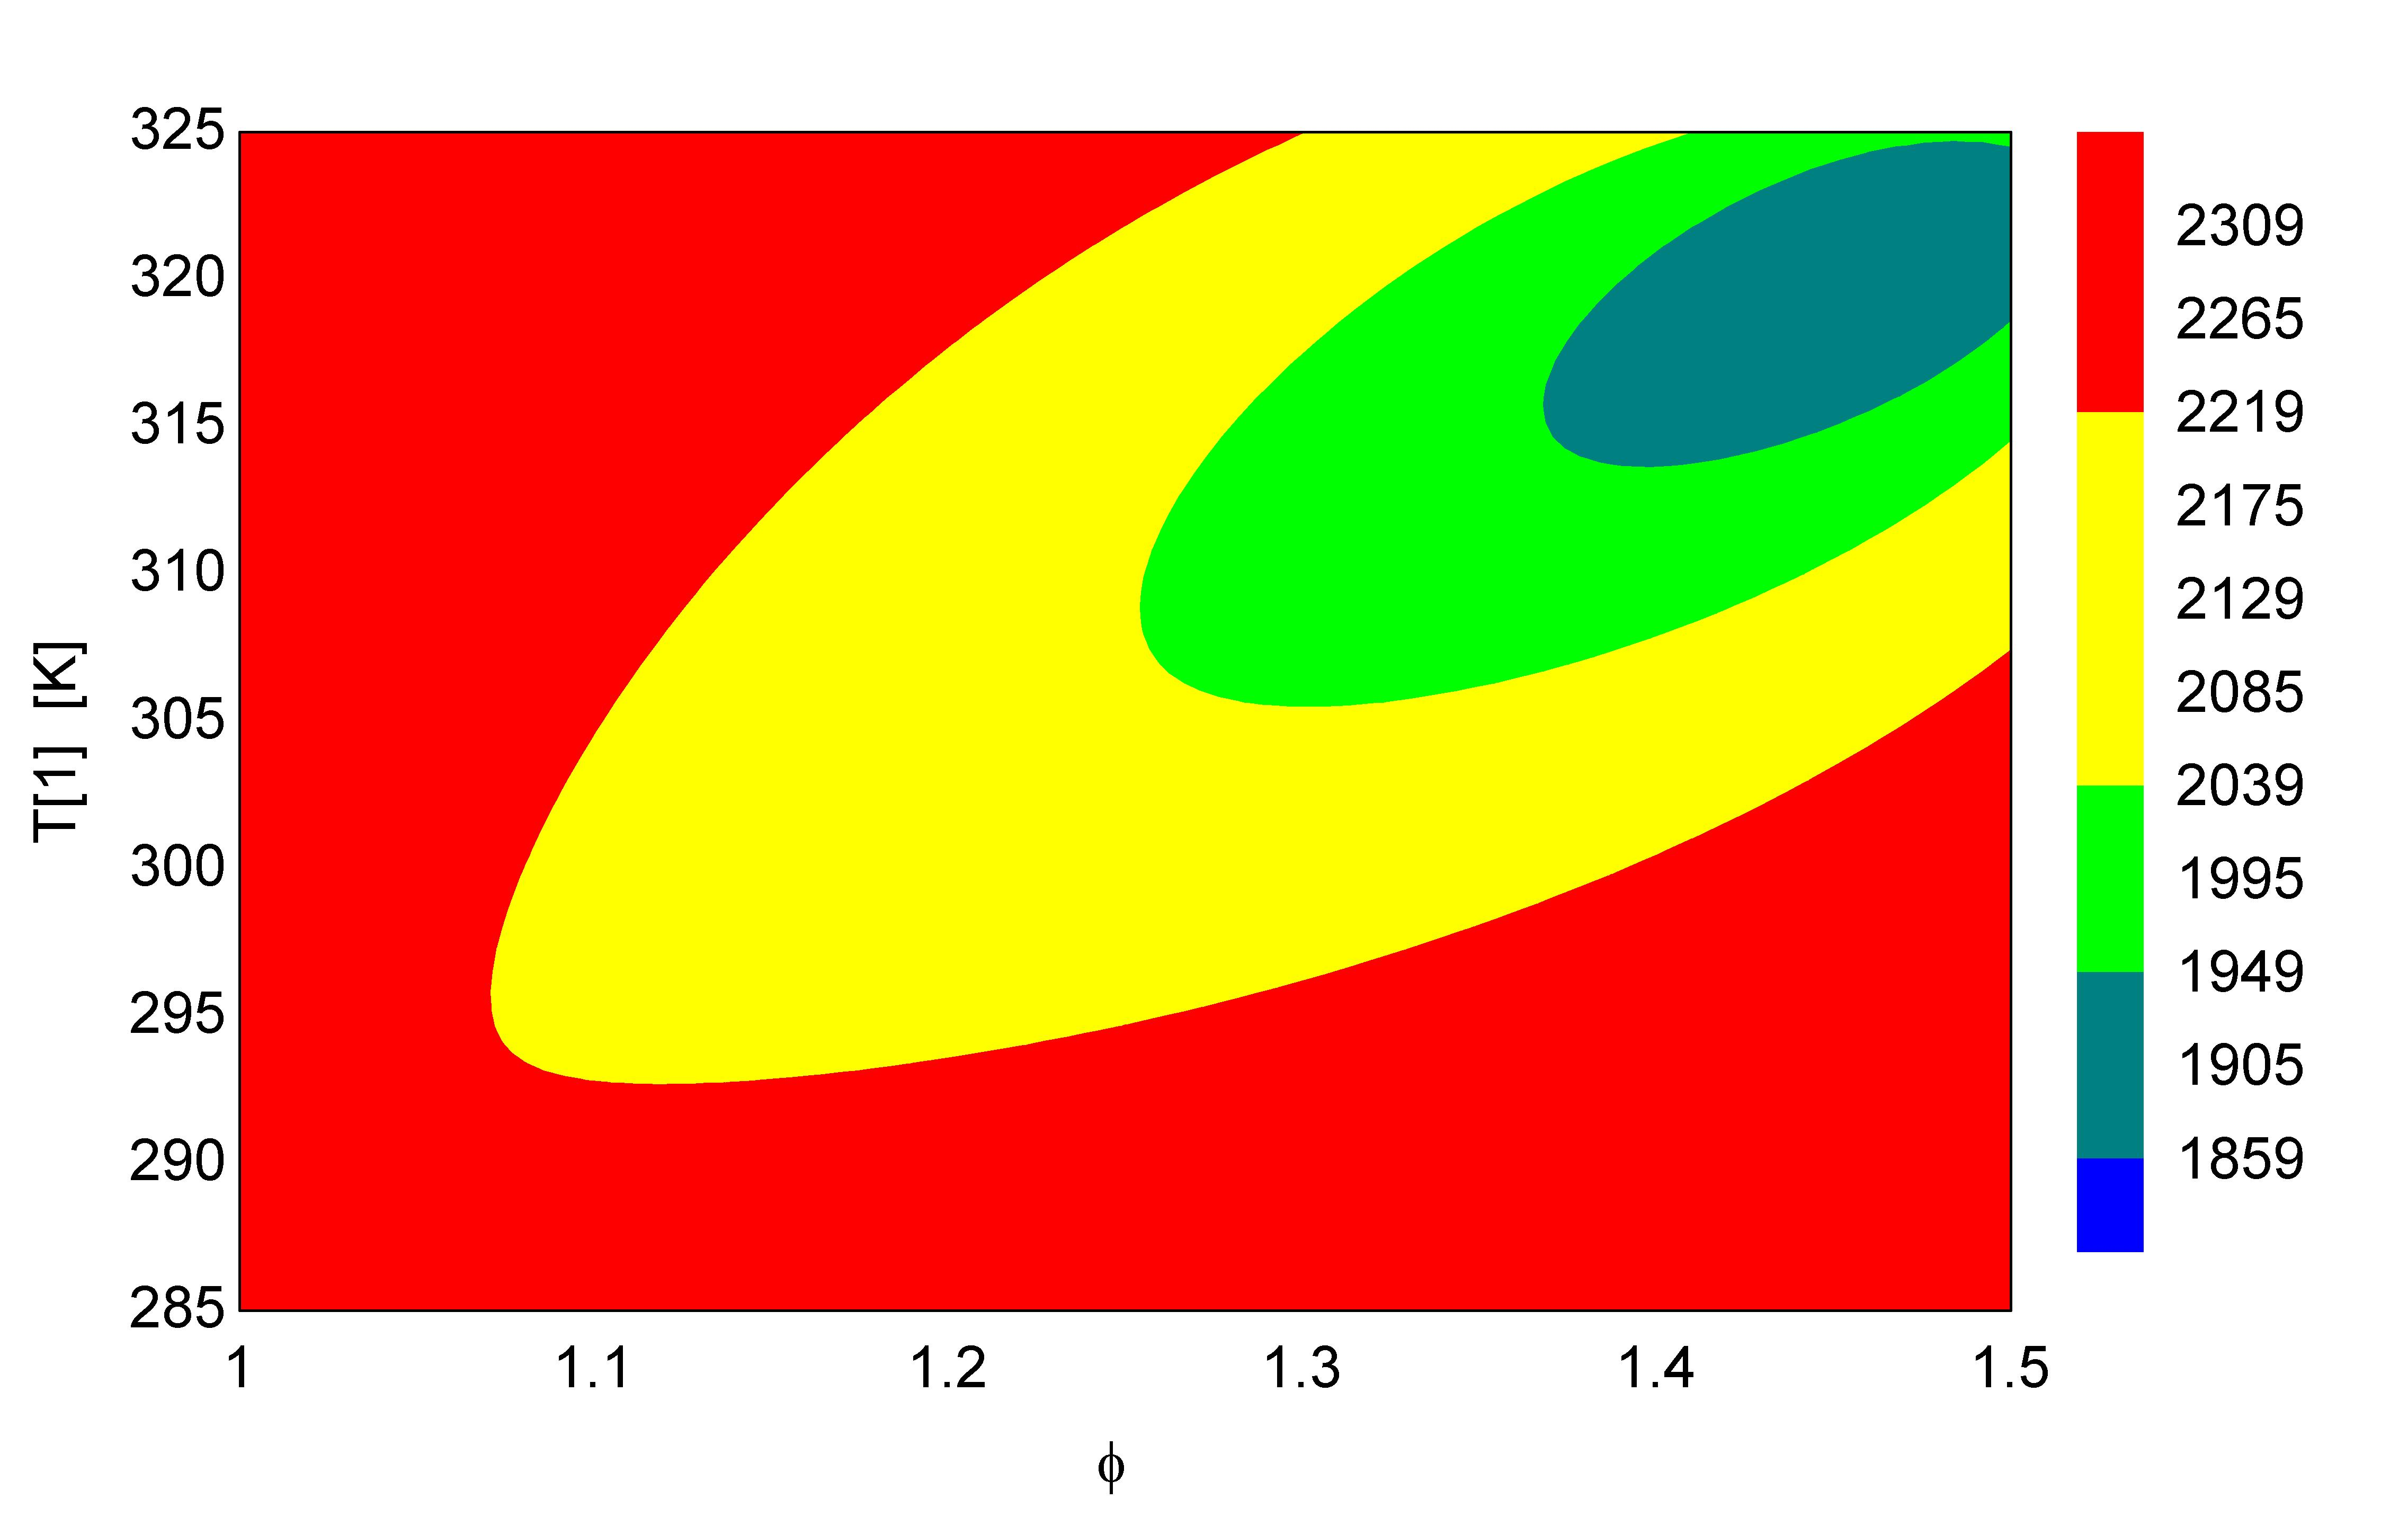
\includegraphics[width=5.0cm,keepaspectratio]{taller1_P1.jpg}}
\subsection*{Plot Window 2:\;T[1]\;vs\;FlameT}
{\centerline{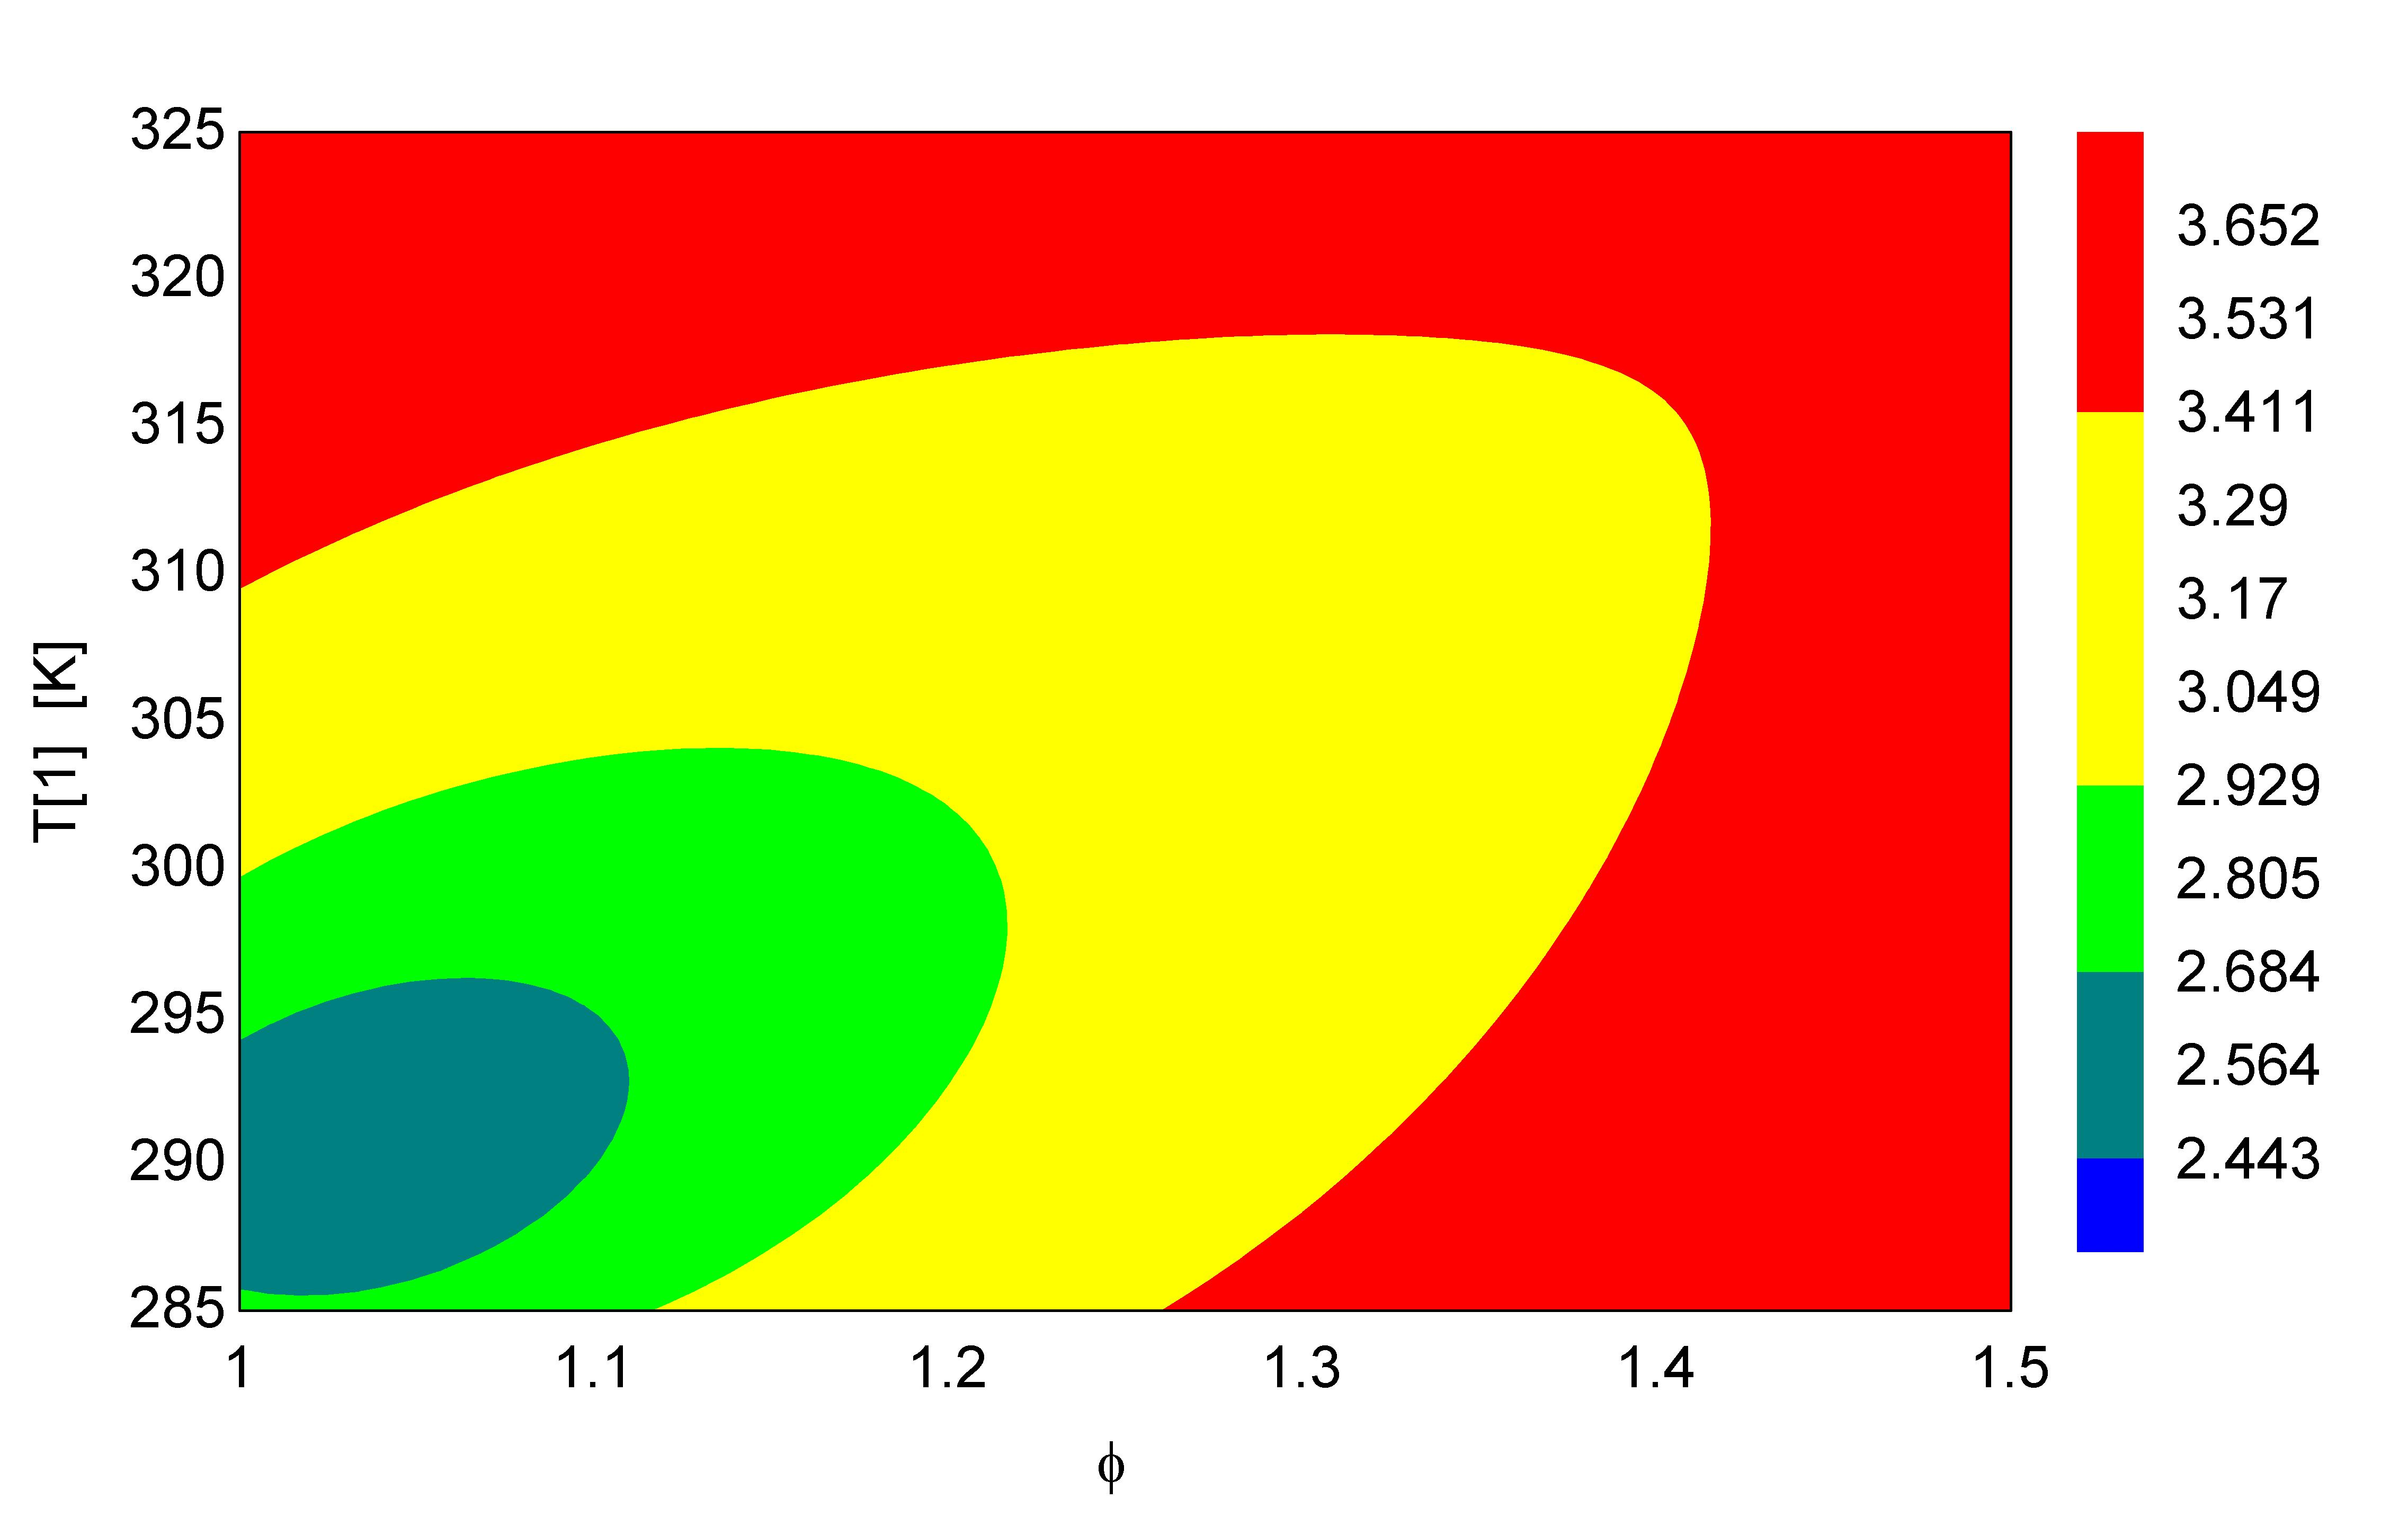
\includegraphics[width=5.0cm,keepaspectratio]{taller1_P2.jpg}}
\subsection*{Plot Window 3:\;ExcessAir\;vs\;Products}
{\centerline{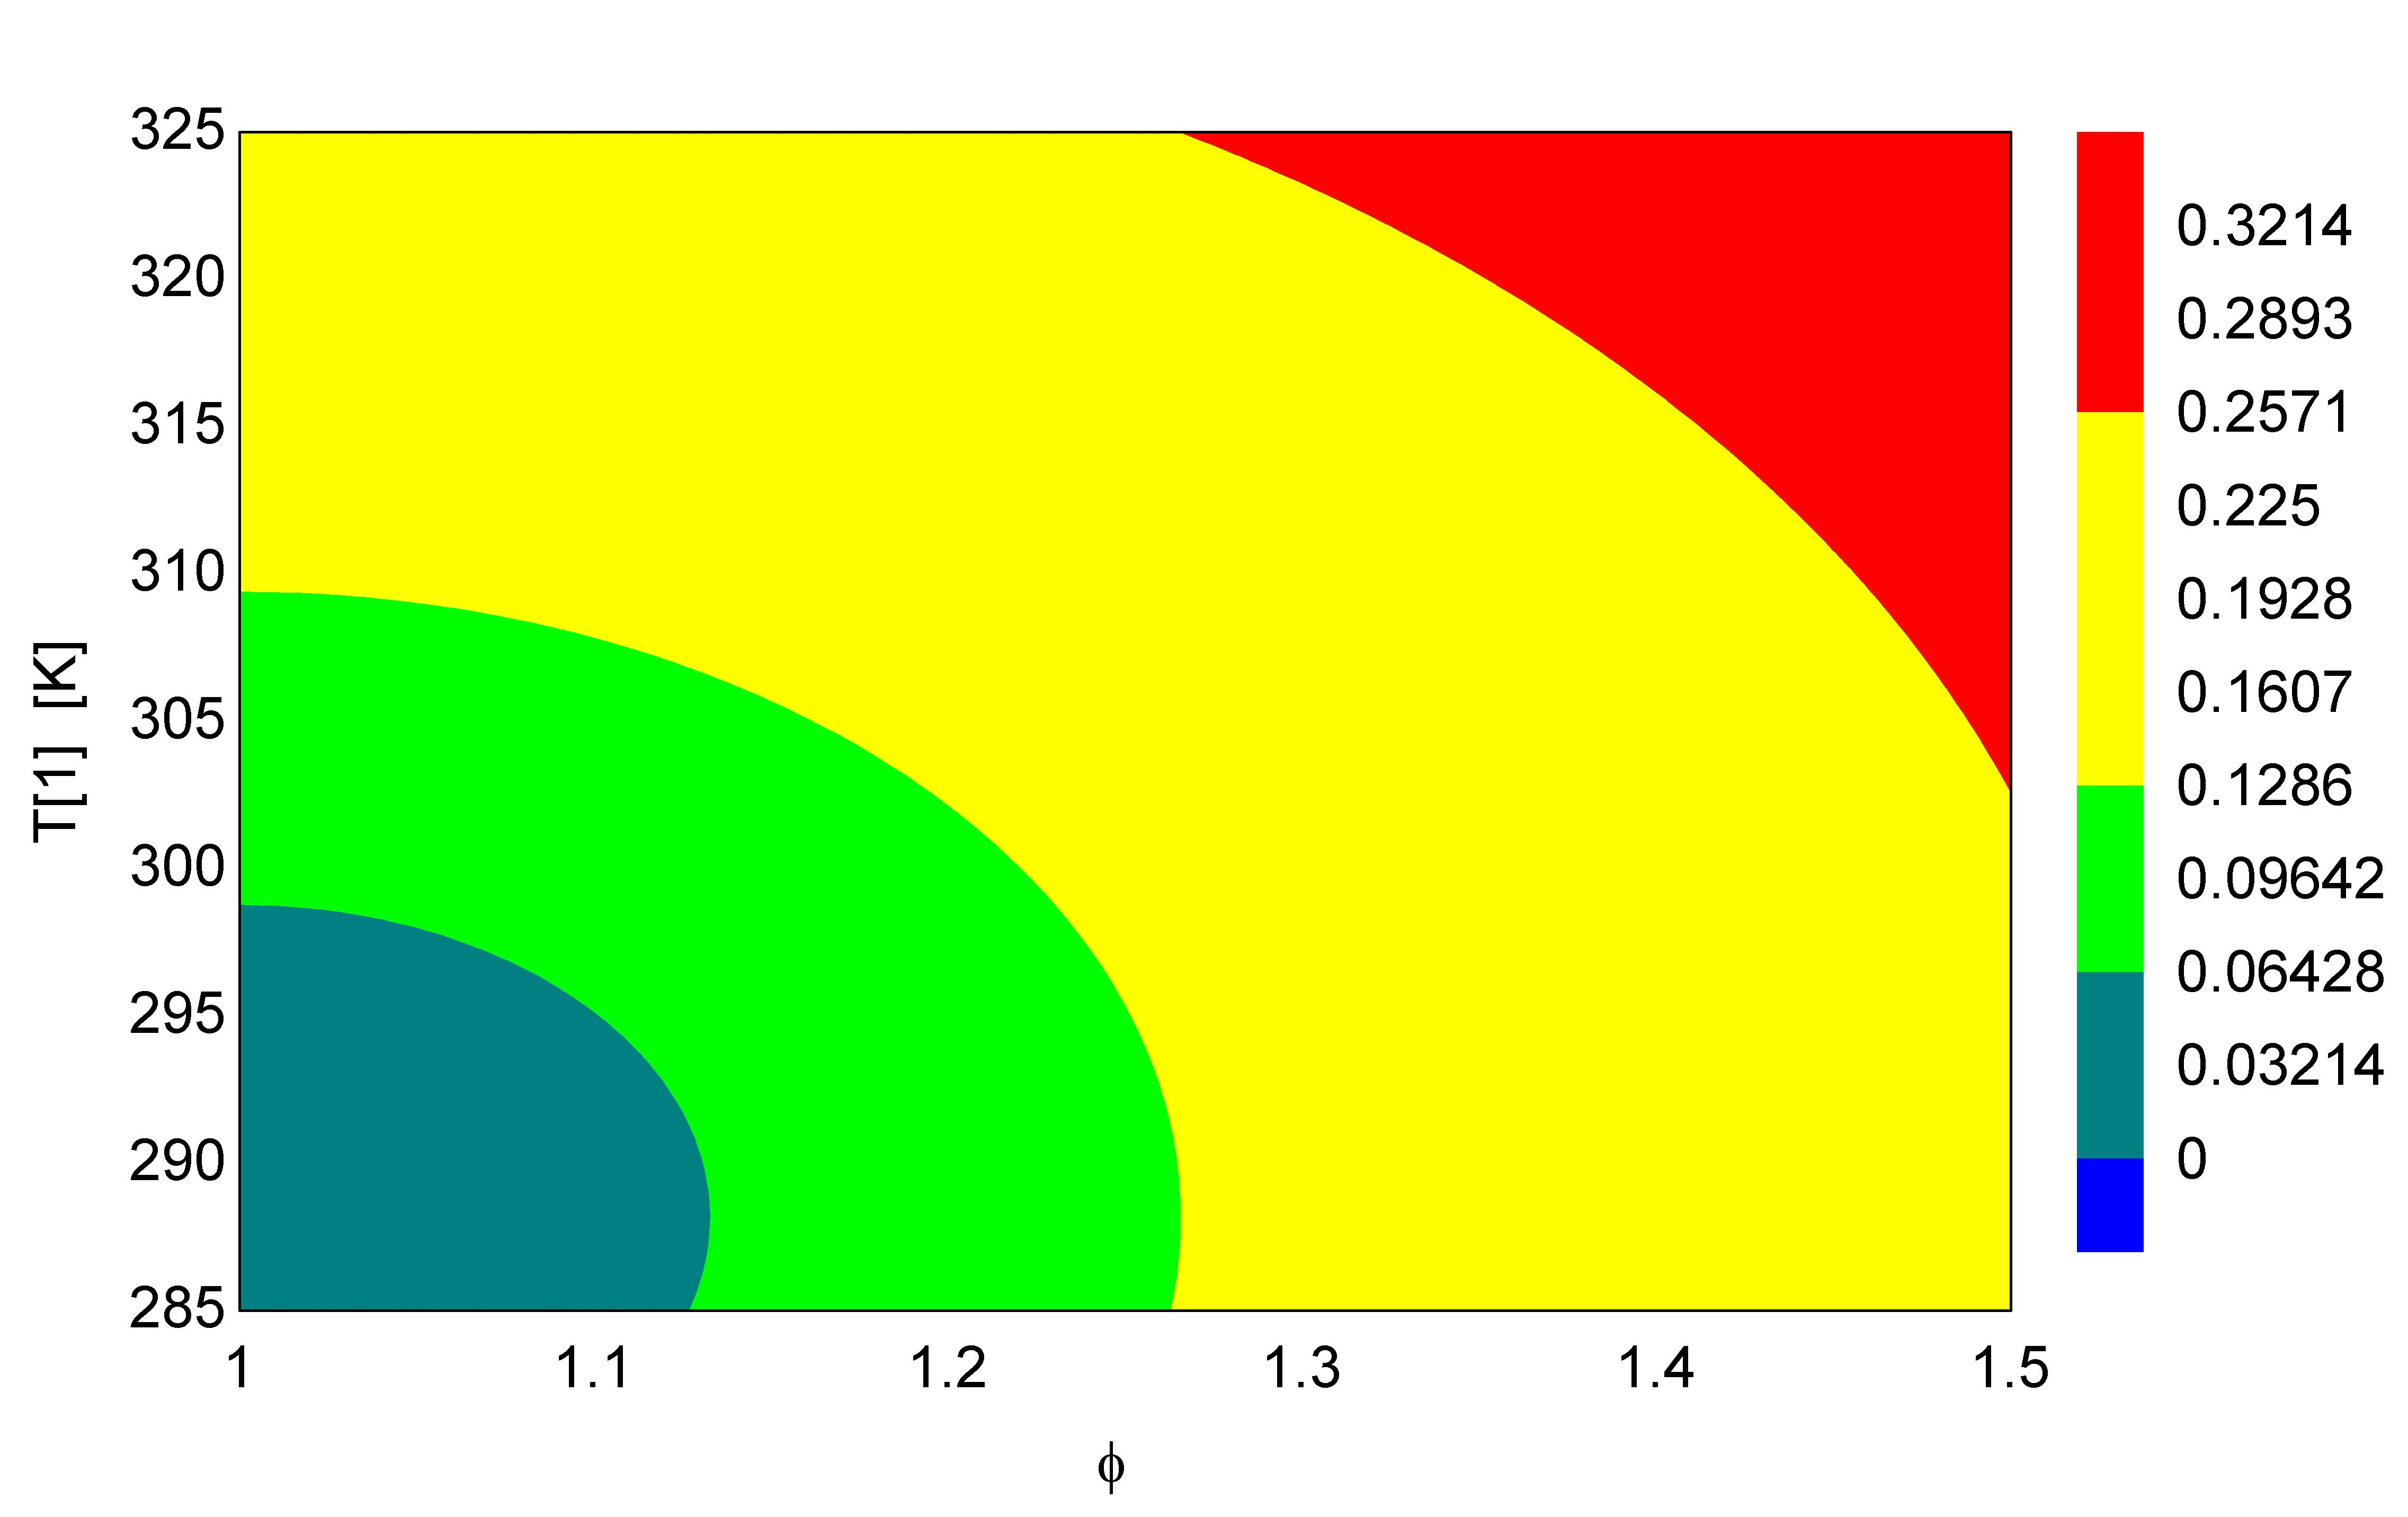
\includegraphics[width=5.0cm,keepaspectratio]{taller1_P3.jpg}}
\subsection*{Plot Window 4:\;T[1]\;vs\;Products}
{\centerline{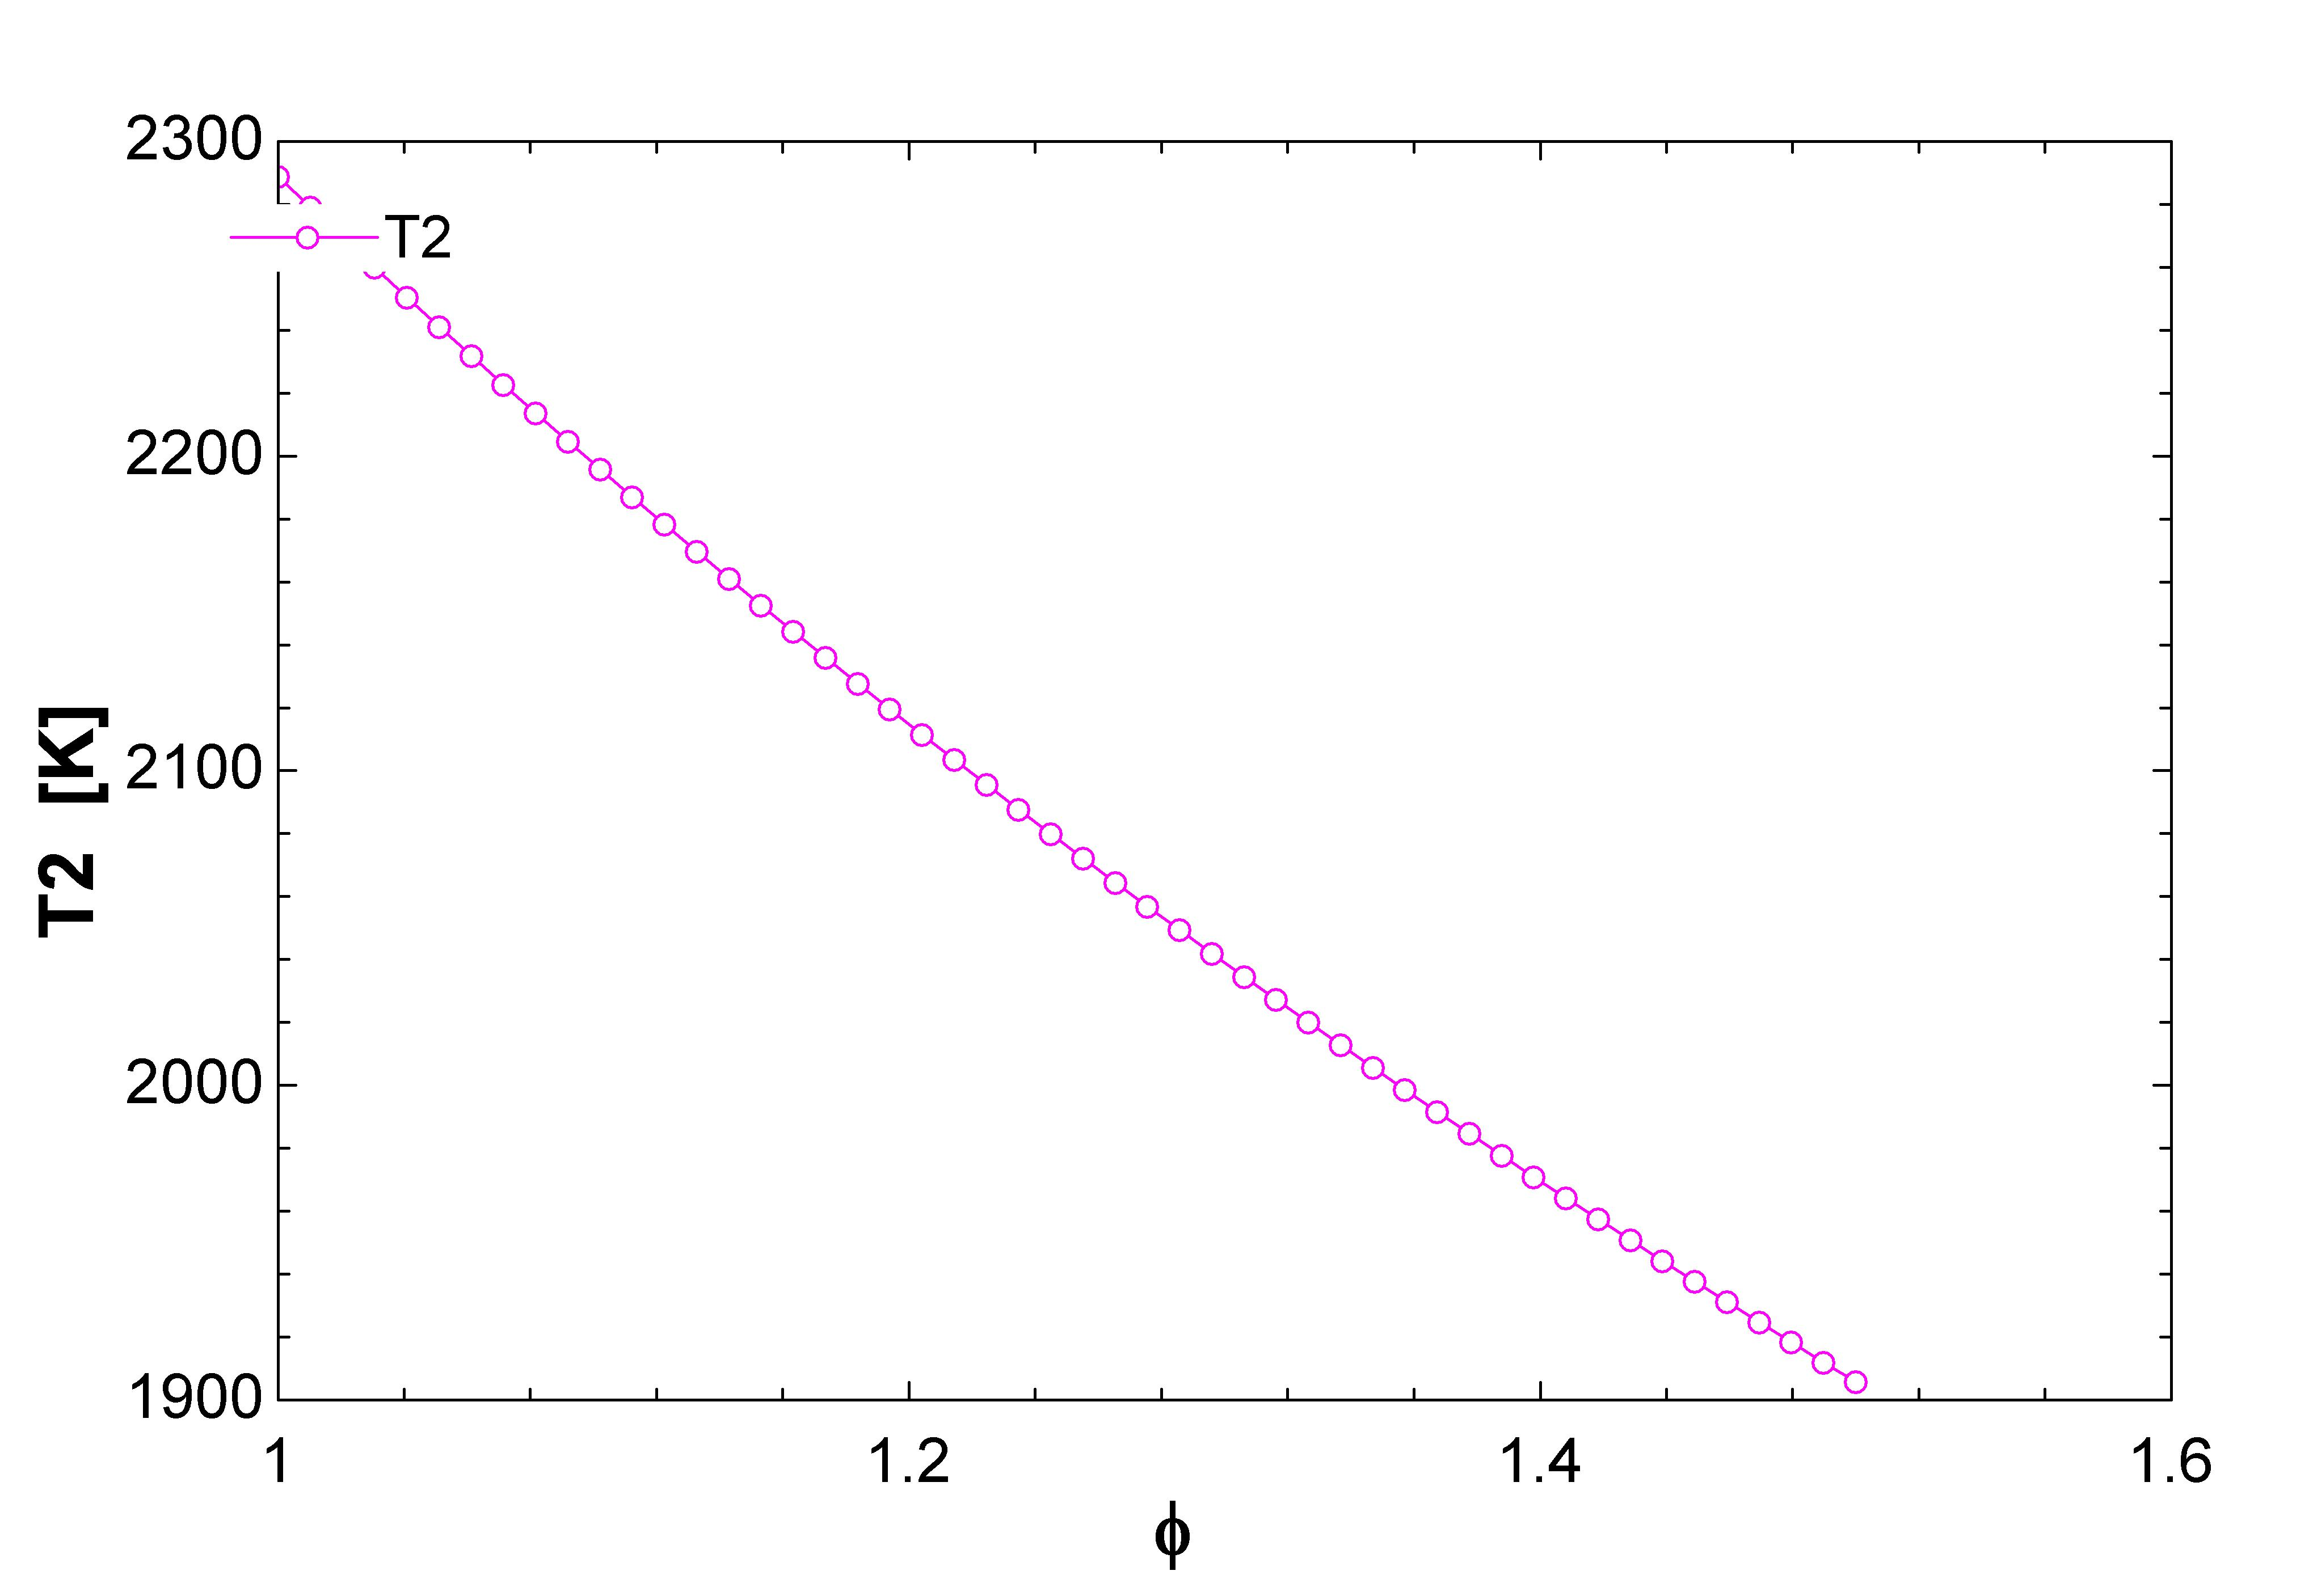
\includegraphics[width=5.0cm,keepaspectratio]{taller1_P4.jpg}}
\end{document}
